\chapter{Binomial Distribution}\label{binomial-distribution}

In statistics, the binomial distribution is a discrete probability of
independent events, where each event has exactly two possible outcomes.
For example, if we toss a coin 10 times and we are interested in how
many times it will land on heads, the probability of it lending one,
two, three, up to 10 head in a row will form a distribution of
probabilities or binomial distribution. When we're interested in a
specific outcome, let's say 3 heads out of 10 tosses, we call it
binomial probability, which is a probability of exactly \(k\) successes
on \(n\) repeated trials.

Following the characteristics of this distribution:

\begin{itemize}
\tightlist
\item
  the number of observations or trials is fixed;
\item
  each observation or trial is independent. Like in the coin toss, the
  previous toss doesn't affect the following;
\item
  the probability of success is exactly the same from one trial to
  another. Each coin toss has 50\% chances to fall in heads or tails.
\end{itemize}

\section{Probability Mass Function}\label{probability-mass-function}

The probabilty mass function in this case describes the
probability of an outcome, and for the binomial distribution is

\begin{equation} \mathrm{PMF}_{\mathrm{binomial}} = \cfrac{n!}{k!(n-k)!}p^k (1-p)^{n-k}
\label{eq:binomial_pmf}
\end{equation}
where \(n\) is the number of observations, \(k\) the desired outcome,
\(p\) the probability of an outcome. To have a better understanding of
how this formula works let's take a look at two examples.

\section{A Fair Coin Flip}\label{a-fair-coin-flip}

If we flip a fair coin 100 times, what is the probability of getting
exactly 50 heads ? Now we might think that since we have equal chances
of getting heads or tails, the answer would be 50\% probability. On the
other hand, what are the odds that we will get 49 heads, or 51 ? Almost
50\% chance too, but what exactly ? Let's first answer the first
question and then try it for all the possible outcomes to see how our
probabilities are distributed. So our parameters are the following:
\(n = 100\), \(k = 50\), \(p = 0.5\). Plugging numbers into Eq.~\ref{eq:binomial_pmf} the formula
and we get

\[P(50) = \cfrac{100!}{50!(100 - 50)!}0.5^{50}(1-0.5)^{(100-50)} \approx 8\% \]

So there is an 8\% chance of getting exactly 50 heads on 100 coin
tosses. The chart below shows how to get this number in \(\tt{python}\)
and the binomial distribution for all possible outcomes. The probability distribution
is shown in Fig.~\ref{fig:binomial_coin_flip}.

\begin{codebox}[breakable, size=fbox, boxrule=1pt, pad at break*=1mm,colback=cellbackground, colframe=cellborder]
\begin{Verbatim}[commandchars=\\\{\}]
\PY{k+kn}{from} \PY{n+nn}{scipy}\PY{n+nn}{.}\PY{n+nn}{stats} \PY{k}{import} \PY{n}{binom}

\PY{n}{b} \PY{o}{=} \PY{n}{binom}\PY{p}{(}\PY{l+m+mi}{100}\PY{p}{,} \PY{l+m+mf}{0.5}\PY{p}{)} \PY{c+c1}{\PYZsh{} params (n, p)}
\PY{n+nb}{print} \PY{p}{(}\PY{l+s+s2}{\PYZdq{}}\PY{l+s+s2}{P(50): }\PY{l+s+si}{\PYZob{}:.2f\PYZcb{}}\PY{l+s+s2}{\PYZpc{}}\PY{l+s+s2}{\PYZdq{}}\PY{o}{.}\PY{n}{format}\PY{p}{(}\PY{n}{b}\PY{o}{.}\PY{n}{pmf}\PY{p}{(}\PY{l+m+mi}{50}\PY{p}{)}\PY{o}{*}\PY{l+m+mi}{100}\PY{p}{)}\PY{p}{)}

P(50): 7.96\%
\end{Verbatim}
\end{codebox}

\begin{figure}[ht]
\centering
    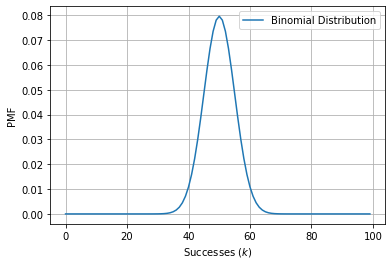
\includegraphics[width=0.7\textwidth]{figures/binomial_2_0.png}
    \caption{Binomial distribution relative to 100 coin flips.}
    \label{fig:binomial_coin_flip}
\end{figure}
    
\section{Success of Marketing Campaign}\label{success-of-marketing-campaign}

In 2014, 8.5\% of adults aged 18 years and older had diabetes. Let's go
back to 2014 and pretend we're working for the company that developed a
drug for treating diabetes and our job is to make phone calls to find
potential clients. The only statistic we know is that 8.5\% of adults in
the US have diabetes. What is the probability that out of 50 calls at
least 5 customers would have diabetes ? Once again let's plug numbers
into the formula: \(n = 50\), \(k > 5\), \(p = 0.085\)

\[\sum_{k=5}^{n}P(k) = \sum_{k=5}^{n}\Big(\cfrac{50!}{k!(50 - k)!}0.085^{k}(1-0.085)^{(50-k)}\Big) \approx 42.2\% \]
there is a 42.2\% chance that out of 50 calls we will find at least five
customers with diabetes. Again in \(\tt{python}\), this time instead of
summing PMFs we exploit the binomial CDF (see Fig.~\ref{fig:binomial_cdf})

\begin{codebox}[breakable, size=fbox, boxrule=1pt, pad at break*=1mm,colback=cellbackground, colframe=cellborder]
\begin{Verbatim}[commandchars=\\\{\}]
\PY{n}{b} \PY{o}{=} \PY{n}{binom}\PY{p}{(}\PY{l+m+mi}{50}\PY{p}{,} \PY{l+m+mf}{0.085}\PY{p}{)} \PY{c+c1}{\PYZsh{} params (n, p)}
\PY{n}{prob} \PY{o}{=} \PY{n}{b}\PY{o}{.}\PY{n}{cdf}\PY{p}{(}\PY{l+m+mi}{50}\PY{p}{)}\PY{o}{\PYZhy{}}\PY{n}{b}\PY{o}{.}\PY{n}{cdf}\PY{p}{(}\PY{l+m+mi}{4}\PY{p}{)}s
\PY{n+nb}{print} \PY{p}{(}\PY{l+s+s2}{\PYZdq{}}\PY{l+s+s2}{P(\PYZgt{}=5): }\PY{l+s+si}{\PYZob{}:.1f\PYZcb{}}\PY{l+s+s2}{\PYZpc{}}\PY{l+s+s2}{\PYZdq{}}\PY{o}{.}\PY{n}{format}\PY{p}{(}\PY{n}{prob}\PY{o}{*}\PY{l+m+mi}{100}\PY{p}{)}\PY{p}{)}

P(>=5): 42.2\%
\end{Verbatim}
\end{codebox}

    \begin{figure}[htb]
    \centering
    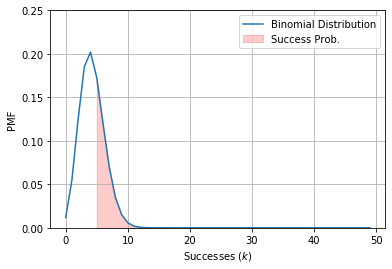
\includegraphics[width=0.7\textwidth]{figures/binomial_5_0.png}
    \caption{Binomial distribution of 50 calls with ($p=0.085$), in red the integrated probability of finding 5 or more successes.}
    \label{fig:binomial_cdf}
    \end{figure}
    